ระบบจำแนกการกระทำของมนุษย์\textsuperscript{\cite{ma2017less}}เป็นหัวข้อที่มีการให้ความสนใจอย่างมากสำหรับการทำระบบประมวลผลวิดีโอในปัจจุบัน เนื่องจากระบบประมวลผลวิดีโอนั้นสามารถใช้งานได้หลากหลายสถานการณ์ เช่น ใช้สอดส่องการจราจรบนท้องถนน
วิเคราะห์พฤติกรรมการเคลื่อนที่ของลูกค้าภายในห้าง การตามหาคนหายหรือพลัดหลงภายในอาคาร เป็นต้น ซึ่งการที่ระบบสามารถจำแนกการกระทำของมนุษย์ภายในวิดีโอได้นั้นสามารถเพิ่มความสามารถของระบบประมวลผลวิดีโอได้
เช่น สามารถแจ้งเตือนเมื่อพบบุคคลที่มีพฤติกรรมน่าสงสัยในวิดีโอได้ เพื่อไม่ให้เกิดเหตุการณ์อันตรายขึ้น เป็นต้น

\begin{figure}[!ht]
	\centering
	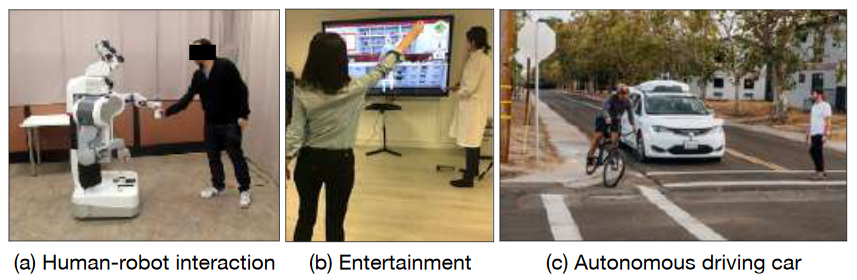
\includegraphics[width=0.6\textwidth]{chapter2/images/video_analytics_ex.png}
	\caption{ตัวอย่างการประยุกต์ใช้งานระบบจำแนกการกระทำมนุษย์\textsuperscript{\cite{kong2018human}}}
	\label{fig:actioncls_ex}
\end{figure}

การสร้างโมเดลปัญญาประดิษฐ์สำหรับจำแนกการกระทำนั้น จำเป็นต้องมีชุดข้อมูลที่เหมาะสมกับการกระทำที่สนใจ และโครงสร้างโมเดลปัญญาประดิษฐ์ที่เหมาะสม
ซึ่งในปัจจุบันนั้นมีชุดข้อมูลสาธารณะที่สามารถนำมาใช้งานได้หลากหลายชุดข้อมูล เช่น YouTube-8M ชุดข้อมูลสำหรับการประมวลผลวิดีโอที่มีขนาดใหญ่ที่สุดและมีจำนวนคำกำกับมากที่สุด, 
AVA ชุดข้อมูลของการกระทำที่มีการขยับเพียงเล็กน้อย, Sports-1M\textsuperscript{\cite{karpathy2014large}} ชุดข้อมูลที่เกี่ยวกับกิจกรรมกีฬาต่างๆของมนุษย์ เป็นต้น ซึ่งชุดข้อมูลที่ผู้วิจัยเลือกนำมาศึกษาได้แก่ YouTube-8M, AVA และ Moment in Time
โดยแต่ละชุดข้อมูลจะมีความแตกต่างกันในหลายๆด้านแต่จะมีสิ่งที่เหมือนกัน คือ เป็นชุดข้อมูลสำหรับการวิเคราะห์วิดีโอที่สนใจการกระทำและกิจกรรมของมนุษย์ โดยจะกล่าวถึงความแตกต่างในด้านต่างๆ 
เช่น เป้าหมายของแต่ละชุดข้อมูล วิธีการเก็บข้อมูลสำหรับชุดข้อมูล วิธีการสร้างคำกำกับ และรายละเอียดอื่นๆของชุดข้อมูล จากนั้นจะสรุปข้อมูลของแต่ละชุดข้อมูลในหัวข้อที่ \ref{sec:dataset}